\documentclass[twoside]{book}

% Packages required by doxygen
\usepackage{fixltx2e}
\usepackage{calc}
\usepackage{doxygen}
\usepackage[export]{adjustbox} % also loads graphicx
\usepackage{graphicx}
\usepackage[utf8]{inputenc}
\usepackage{makeidx}
\usepackage{multicol}
\usepackage{multirow}
\PassOptionsToPackage{warn}{textcomp}
\usepackage{textcomp}
\usepackage[nointegrals]{wasysym}
\usepackage[table]{xcolor}

% Font selection
\usepackage[T1]{fontenc}
\usepackage[scaled=.90]{helvet}
\usepackage{courier}
\usepackage{amssymb}
\usepackage{sectsty}
\renewcommand{\familydefault}{\sfdefault}
\allsectionsfont{%
  \fontseries{bc}\selectfont%
  \color{darkgray}%
}
\renewcommand{\DoxyLabelFont}{%
  \fontseries{bc}\selectfont%
  \color{darkgray}%
}
\newcommand{\+}{\discretionary{\mbox{\scriptsize$\hookleftarrow$}}{}{}}

% Page & text layout
\usepackage{geometry}
\geometry{%
  a4paper,%
  top=2.5cm,%
  bottom=2.5cm,%
  left=2.5cm,%
  right=2.5cm%
}
\tolerance=750
\hfuzz=15pt
\hbadness=750
\setlength{\emergencystretch}{15pt}
\setlength{\parindent}{0cm}
\setlength{\parskip}{3ex plus 2ex minus 2ex}
\makeatletter
\renewcommand{\paragraph}{%
  \@startsection{paragraph}{4}{0ex}{-1.0ex}{1.0ex}{%
    \normalfont\normalsize\bfseries\SS@parafont%
  }%
}
\renewcommand{\subparagraph}{%
  \@startsection{subparagraph}{5}{0ex}{-1.0ex}{1.0ex}{%
    \normalfont\normalsize\bfseries\SS@subparafont%
  }%
}
\makeatother

% Headers & footers
\usepackage{fancyhdr}
\pagestyle{fancyplain}
\fancyhead[LE]{\fancyplain{}{\bfseries\thepage}}
\fancyhead[CE]{\fancyplain{}{}}
\fancyhead[RE]{\fancyplain{}{\bfseries\leftmark}}
\fancyhead[LO]{\fancyplain{}{\bfseries\rightmark}}
\fancyhead[CO]{\fancyplain{}{}}
\fancyhead[RO]{\fancyplain{}{\bfseries\thepage}}
\fancyfoot[LE]{\fancyplain{}{}}
\fancyfoot[CE]{\fancyplain{}{}}
\fancyfoot[RE]{\fancyplain{}{\bfseries\scriptsize Generated by Doxygen }}
\fancyfoot[LO]{\fancyplain{}{\bfseries\scriptsize Generated by Doxygen }}
\fancyfoot[CO]{\fancyplain{}{}}
\fancyfoot[RO]{\fancyplain{}{}}
\renewcommand{\footrulewidth}{0.4pt}
\renewcommand{\chaptermark}[1]{%
  \markboth{#1}{}%
}
\renewcommand{\sectionmark}[1]{%
  \markright{\thesection\ #1}%
}

% Indices & bibliography
\usepackage{natbib}
\usepackage[titles]{tocloft}
\setcounter{tocdepth}{3}
\setcounter{secnumdepth}{5}
\makeindex

% Hyperlinks (required, but should be loaded last)
\usepackage{ifpdf}
\ifpdf
  \usepackage[pdftex,pagebackref=true]{hyperref}
\else
  \usepackage[ps2pdf,pagebackref=true]{hyperref}
\fi
\hypersetup{%
  colorlinks=true,%
  linkcolor=blue,%
  citecolor=blue,%
  unicode%
}

% Custom commands
\newcommand{\clearemptydoublepage}{%
  \newpage{\pagestyle{empty}\cleardoublepage}%
}

\usepackage{caption}
\captionsetup{labelsep=space,justification=centering,font={bf},singlelinecheck=off,skip=4pt,position=top}

%===== C O N T E N T S =====

\begin{document}

% Titlepage & ToC
\hypersetup{pageanchor=false,
             bookmarksnumbered=true,
             pdfencoding=unicode
            }
\pagenumbering{roman}
\begin{titlepage}
\vspace*{7cm}
\begin{center}%
{\Large Circuit Simulator }\\
\vspace*{1cm}
{\large Generated by Doxygen 1.8.11}\\
\end{center}
\end{titlepage}
\clearemptydoublepage
\tableofcontents
\clearemptydoublepage
\pagenumbering{arabic}
\hypersetup{pageanchor=true}

%--- Begin generated contents ---
\chapter{Namespace Index}
\section{Namespace List}
Here is a list of all namespaces with brief descriptions\+:\begin{DoxyCompactList}
\item\contentsline{section}{\hyperlink{namespacecisim}{cisim} }{\pageref{namespacecisim}}{}
\item\contentsline{section}{\hyperlink{namespacecisim_1_1nodes}{cisim\+::nodes} }{\pageref{namespacecisim_1_1nodes}}{}
\end{DoxyCompactList}

\chapter{Hierarchical Index}
\section{Class Hierarchy}
This inheritance list is sorted roughly, but not completely, alphabetically\+:\begin{DoxyCompactList}
\item \contentsline{section}{cisim\+:\+:Circuit}{\pageref{classcisim_1_1_circuit}}{}
\item \contentsline{section}{Circuit\+Simulator}{\pageref{class_circuit_simulator}}{}
\item \contentsline{section}{cisim\+:\+:nodes\+:\+:Node}{\pageref{classcisim_1_1nodes_1_1_node}}{}
\begin{DoxyCompactList}
\item \contentsline{section}{cisim\+:\+:nodes\+:\+:And\+Node}{\pageref{classcisim_1_1nodes_1_1_and_node}}{}
\item \contentsline{section}{cisim\+:\+:nodes\+:\+:Input\+Node}{\pageref{classcisim_1_1nodes_1_1_input_node}}{}
\item \contentsline{section}{cisim\+:\+:nodes\+:\+:Nand\+Node}{\pageref{classcisim_1_1nodes_1_1_nand_node}}{}
\item \contentsline{section}{cisim\+:\+:nodes\+:\+:Nor\+Node}{\pageref{classcisim_1_1nodes_1_1_nor_node}}{}
\item \contentsline{section}{cisim\+:\+:nodes\+:\+:Not\+Node}{\pageref{classcisim_1_1nodes_1_1_not_node}}{}
\item \contentsline{section}{cisim\+:\+:nodes\+:\+:Or\+Node}{\pageref{classcisim_1_1nodes_1_1_or_node}}{}
\item \contentsline{section}{cisim\+:\+:nodes\+:\+:Xor\+Node}{\pageref{classcisim_1_1nodes_1_1_xor_node}}{}
\end{DoxyCompactList}
\item \contentsline{section}{cisim\+:\+:nodes\+:\+:Node\+Registrar}{\pageref{classcisim_1_1nodes_1_1_node_registrar}}{}
\item \contentsline{section}{cisim\+:\+:nodes\+:\+:Node\+Registrar$<$ cisim\+:\+:nodes\+:\+:And\+Node $>$}{\pageref{classcisim_1_1nodes_1_1_node_registrar}}{}
\item \contentsline{section}{cisim\+:\+:nodes\+:\+:Node\+Registrar$<$ cisim\+:\+:nodes\+:\+:Input\+Node $>$}{\pageref{classcisim_1_1nodes_1_1_node_registrar}}{}
\item \contentsline{section}{cisim\+:\+:nodes\+:\+:Node\+Registrar$<$ cisim\+:\+:nodes\+:\+:Nand\+Node $>$}{\pageref{classcisim_1_1nodes_1_1_node_registrar}}{}
\item \contentsline{section}{cisim\+:\+:nodes\+:\+:Node\+Registrar$<$ cisim\+:\+:nodes\+:\+:Nor\+Node $>$}{\pageref{classcisim_1_1nodes_1_1_node_registrar}}{}
\item \contentsline{section}{cisim\+:\+:nodes\+:\+:Node\+Registrar$<$ cisim\+:\+:nodes\+:\+:Not\+Node $>$}{\pageref{classcisim_1_1nodes_1_1_node_registrar}}{}
\item \contentsline{section}{cisim\+:\+:nodes\+:\+:Node\+Registrar$<$ cisim\+:\+:nodes\+:\+:Or\+Node $>$}{\pageref{classcisim_1_1nodes_1_1_node_registrar}}{}
\item \contentsline{section}{cisim\+:\+:nodes\+:\+:Node\+Registrar$<$ cisim\+:\+:nodes\+:\+:Xor\+Node $>$}{\pageref{classcisim_1_1nodes_1_1_node_registrar}}{}
\item Singleton\begin{DoxyCompactList}
\item \contentsline{section}{cisim\+:\+:nodes\+:\+:Node\+Factory}{\pageref{classcisim_1_1nodes_1_1_node_factory}}{}
\end{DoxyCompactList}
\end{DoxyCompactList}

\chapter{Class Index}
\section{Class List}
Here are the classes, structs, unions and interfaces with brief descriptions\+:\begin{DoxyCompactList}
\item\contentsline{section}{\hyperlink{classcisim_1_1_circuit}{cisim\+::\+Circuit} \\*\hyperlink{classcisim_1_1_circuit}{Circuit} class }{\pageref{classcisim_1_1_circuit}}{}
\item\contentsline{section}{\hyperlink{classcisim_1_1_circuit_simulator}{cisim\+::\+Circuit\+Simulator} \\*Application class }{\pageref{classcisim_1_1_circuit_simulator}}{}
\item\contentsline{section}{\hyperlink{classcisim_1_1nodes_1_1_node}{cisim\+::nodes\+::\+Node} }{\pageref{classcisim_1_1nodes_1_1_node}}{}
\item\contentsline{section}{\hyperlink{classcisim_1_1nodes_1_1_node_factory}{cisim\+::nodes\+::\+Node\+Factory} }{\pageref{classcisim_1_1nodes_1_1_node_factory}}{}
\item\contentsline{section}{\hyperlink{classcisim_1_1nodes_1_1_node_registrar}{cisim\+::nodes\+::\+Node\+Registrar} }{\pageref{classcisim_1_1nodes_1_1_node_registrar}}{}
\end{DoxyCompactList}

\chapter{File Index}
\section{File List}
Here is a list of all files with brief descriptions\+:\begin{DoxyCompactList}
\item\contentsline{section}{src/\hyperlink{circuitsimulator_8cpp}{circuitsimulator.\+cpp} }{\pageref{circuitsimulator_8cpp}}{}
\item\contentsline{section}{src/\hyperlink{circuitsimulator_8h}{circuitsimulator.\+h} }{\pageref{circuitsimulator_8h}}{}
\item\contentsline{section}{src/\hyperlink{main_8cpp}{main.\+cpp} }{\pageref{main_8cpp}}{}
\item\contentsline{section}{src/\hyperlink{main_8h}{main.\+h} }{\pageref{main_8h}}{}
\item\contentsline{section}{src/cisim/\hyperlink{circuit_8cpp}{circuit.\+cpp} }{\pageref{circuit_8cpp}}{}
\item\contentsline{section}{src/cisim/\hyperlink{circuit_8h}{circuit.\+h} }{\pageref{circuit_8h}}{}
\item\contentsline{section}{src/cisim/nodes/\hyperlink{andnode_8h}{andnode.\+h} }{\pageref{andnode_8h}}{}
\item\contentsline{section}{src/cisim/nodes/\hyperlink{inputnode_8h}{inputnode.\+h} }{\pageref{inputnode_8h}}{}
\item\contentsline{section}{src/cisim/nodes/\hyperlink{nandnode_8h}{nandnode.\+h} }{\pageref{nandnode_8h}}{}
\item\contentsline{section}{src/cisim/nodes/\hyperlink{node_8cpp}{node.\+cpp} }{\pageref{node_8cpp}}{}
\item\contentsline{section}{src/cisim/nodes/\hyperlink{node_8h}{node.\+h} }{\pageref{node_8h}}{}
\item\contentsline{section}{src/cisim/nodes/\hyperlink{nodefactory_8cpp}{nodefactory.\+cpp} }{\pageref{nodefactory_8cpp}}{}
\item\contentsline{section}{src/cisim/nodes/\hyperlink{nodefactory_8h}{nodefactory.\+h} }{\pageref{nodefactory_8h}}{}
\item\contentsline{section}{src/cisim/nodes/\hyperlink{noderegistrar_8cpp}{noderegistrar.\+cpp} }{\pageref{noderegistrar_8cpp}}{}
\item\contentsline{section}{src/cisim/nodes/\hyperlink{noderegistrar_8h}{noderegistrar.\+h} }{\pageref{noderegistrar_8h}}{}
\item\contentsline{section}{src/cisim/nodes/\hyperlink{nornode_8h}{nornode.\+h} }{\pageref{nornode_8h}}{}
\item\contentsline{section}{src/cisim/nodes/\hyperlink{notnode_8h}{notnode.\+h} }{\pageref{notnode_8h}}{}
\item\contentsline{section}{src/cisim/nodes/\hyperlink{ornode_8h}{ornode.\+h} }{\pageref{ornode_8h}}{}
\item\contentsline{section}{src/cisim/nodes/\hyperlink{xornode_8h}{xornode.\+h} }{\pageref{xornode_8h}}{}
\end{DoxyCompactList}

\chapter{Namespace Documentation}
\hypertarget{namespacecisim}{}\section{cisim Namespace Reference}
\label{namespacecisim}\index{cisim@{cisim}}
\subsection*{Namespaces}
\begin{DoxyCompactItemize}
\item 
 \hyperlink{namespacecisim_1_1nodes}{nodes}
\end{DoxyCompactItemize}
\subsection*{Classes}
\begin{DoxyCompactItemize}
\item 
class \hyperlink{classcisim_1_1_circuit}{Circuit}
\begin{DoxyCompactList}\small\item\em \hyperlink{classcisim_1_1_circuit}{Circuit} class. \end{DoxyCompactList}\end{DoxyCompactItemize}
\subsection*{Functions}
\begin{DoxyCompactItemize}
\item 
std\+::istream \& \hyperlink{namespacecisim_a9489303a86fdb03e3f7e13762bd748bd}{operator$>$$>$} (std\+::istream \&istream, \hyperlink{classcisim_1_1_circuit}{Circuit} \&circuit)
\end{DoxyCompactItemize}


\subsection{Function Documentation}
\index{cisim@{cisim}!operator$>$$>$@{operator$>$$>$}}
\index{operator$>$$>$@{operator$>$$>$}!cisim@{cisim}}
\subsubsection[{\texorpdfstring{operator$>$$>$(std\+::istream \&istream, Circuit \&circuit)}{operator>>(std::istream &istream, Circuit &circuit)}}]{\setlength{\rightskip}{0pt plus 5cm}std\+::istream \& cisim\+::operator$>$$>$ (
\begin{DoxyParamCaption}
\item[{std\+::istream \&}]{istream, }
\item[{{\bf Circuit} \&}]{circuit}
\end{DoxyParamCaption}
)}\hypertarget{namespacecisim_a9489303a86fdb03e3f7e13762bd748bd}{}\label{namespacecisim_a9489303a86fdb03e3f7e13762bd748bd}
Parses an input stream into a \hyperlink{classcisim_1_1_circuit}{Circuit} object.


\begin{DoxyParams}{Parameters}
{\em circuit} & A reference to a \hyperlink{classcisim_1_1_circuit}{Circuit} object buffer. \\
\hline
\end{DoxyParams}
\begin{DoxyReturn}{Returns}
A reference to the istream object. 
\end{DoxyReturn}

\hypertarget{namespacecisim_1_1nodes}{}\section{cisim\+:\+:nodes Namespace Reference}
\label{namespacecisim_1_1nodes}\index{cisim\+::nodes@{cisim\+::nodes}}
\subsection*{Classes}
\begin{DoxyCompactItemize}
\item 
class \hyperlink{classcisim_1_1nodes_1_1_node}{Node}
\item 
class \hyperlink{classcisim_1_1nodes_1_1_node_factory}{Node\+Factory}
\item 
class \hyperlink{classcisim_1_1nodes_1_1_node_registrar}{Node\+Registrar}
\end{DoxyCompactItemize}
\subsection*{Functions}
\begin{DoxyCompactItemize}
\item 
std\+::istream \& \hyperlink{namespacecisim_1_1nodes_a80da9ab6657bee6f2f7baa7e7cbc09ba}{operator$>$$>$} (std\+::istream \&istream, \hyperlink{classcisim_1_1nodes_1_1_node}{Node} \&node)
\end{DoxyCompactItemize}


\subsection{Function Documentation}
\index{cisim\+::nodes@{cisim\+::nodes}!operator$>$$>$@{operator$>$$>$}}
\index{operator$>$$>$@{operator$>$$>$}!cisim\+::nodes@{cisim\+::nodes}}
\subsubsection[{\texorpdfstring{operator$>$$>$(std\+::istream \&istream, Node \&node)}{operator>>(std::istream &istream, Node &node)}}]{\setlength{\rightskip}{0pt plus 5cm}std\+::istream \& cisim\+::nodes\+::operator$>$$>$ (
\begin{DoxyParamCaption}
\item[{std\+::istream \&}]{istream, }
\item[{{\bf Node} \&}]{node}
\end{DoxyParamCaption}
)}\hypertarget{namespacecisim_1_1nodes_a80da9ab6657bee6f2f7baa7e7cbc09ba}{}\label{namespacecisim_1_1nodes_a80da9ab6657bee6f2f7baa7e7cbc09ba}

\chapter{Class Documentation}
\input{classcisim_1_1nodes_1_1_and_node}
\hypertarget{classcisim_1_1_circuit}{}\section{cisim\+:\+:Circuit Class Reference}
\label{classcisim_1_1_circuit}\index{cisim\+::\+Circuit@{cisim\+::\+Circuit}}


\hyperlink{classcisim_1_1_circuit}{Circuit} class.  




{\ttfamily \#include $<$circuit.\+h$>$}

\subsection*{Friends}
\begin{DoxyCompactItemize}
\item 
std\+::istream \& \hyperlink{classcisim_1_1_circuit_a0a381487e00ea21d54490fbe01b7c3ff}{operator$>$$>$} (std\+::istream \&istream, \hyperlink{classcisim_1_1_circuit}{Circuit} \&circuit)
\end{DoxyCompactItemize}


\subsection{Detailed Description}
\hyperlink{classcisim_1_1_circuit}{Circuit} class. 

This class represents a circuit as given in a circuit file. 

\subsection{Friends And Related Function Documentation}
\index{cisim\+::\+Circuit@{cisim\+::\+Circuit}!operator$>$$>$@{operator$>$$>$}}
\index{operator$>$$>$@{operator$>$$>$}!cisim\+::\+Circuit@{cisim\+::\+Circuit}}
\subsubsection[{\texorpdfstring{operator$>$$>$}{operator>>}}]{\setlength{\rightskip}{0pt plus 5cm}std\+::istream\& operator$>$$>$ (
\begin{DoxyParamCaption}
\item[{std\+::istream \&}]{istream, }
\item[{{\bf Circuit} \&}]{circuit}
\end{DoxyParamCaption}
)\hspace{0.3cm}{\ttfamily [friend]}}\hypertarget{classcisim_1_1_circuit_a0a381487e00ea21d54490fbe01b7c3ff}{}\label{classcisim_1_1_circuit_a0a381487e00ea21d54490fbe01b7c3ff}
Parses an input stream into a \hyperlink{classcisim_1_1_circuit}{Circuit} object.


\begin{DoxyParams}{Parameters}
{\em circuit} & A reference to a \hyperlink{classcisim_1_1_circuit}{Circuit} object buffer. \\
\hline
\end{DoxyParams}
\begin{DoxyReturn}{Returns}
A reference to the istream object. 
\end{DoxyReturn}


The documentation for this class was generated from the following file\+:\begin{DoxyCompactItemize}
\item 
src/cisim/\hyperlink{circuit_8h}{circuit.\+h}\end{DoxyCompactItemize}

\input{class_circuit_simulator}
\input{classcisim_1_1nodes_1_1_input_node}
\input{classcisim_1_1nodes_1_1_nand_node}
\hypertarget{classcisim_1_1nodes_1_1_node}{}\section{cisim\+:\+:nodes\+:\+:Node Class Reference}
\label{classcisim_1_1nodes_1_1_node}\index{cisim\+::nodes\+::\+Node@{cisim\+::nodes\+::\+Node}}


{\ttfamily \#include $<$node.\+h$>$}



Inheritance diagram for cisim\+:\+:nodes\+:\+:Node\+:
\nopagebreak
\begin{figure}[H]
\begin{center}
\leavevmode
\includegraphics[width=350pt]{classcisim_1_1nodes_1_1_node__inherit__graph}
\end{center}
\end{figure}


Collaboration diagram for cisim\+:\+:nodes\+:\+:Node\+:
\nopagebreak
\begin{figure}[H]
\begin{center}
\leavevmode
\includegraphics[width=180pt]{classcisim_1_1nodes_1_1_node__coll__graph}
\end{center}
\end{figure}
\subsection*{Friends}
\begin{DoxyCompactItemize}
\item 
std\+::istream \& \hyperlink{classcisim_1_1nodes_1_1_node_aa3dc9e276e94cce725cb34c8212271cb}{operator$>$$>$} (std\+::istream \&istream, \hyperlink{classcisim_1_1nodes_1_1_node}{Node} \&node)
\end{DoxyCompactItemize}


\subsection{Friends And Related Function Documentation}
\index{cisim\+::nodes\+::\+Node@{cisim\+::nodes\+::\+Node}!operator$>$$>$@{operator$>$$>$}}
\index{operator$>$$>$@{operator$>$$>$}!cisim\+::nodes\+::\+Node@{cisim\+::nodes\+::\+Node}}
\subsubsection[{\texorpdfstring{operator$>$$>$}{operator>>}}]{\setlength{\rightskip}{0pt plus 5cm}std\+::istream\& operator$>$$>$ (
\begin{DoxyParamCaption}
\item[{std\+::istream \&}]{istream, }
\item[{{\bf Node} \&}]{node}
\end{DoxyParamCaption}
)\hspace{0.3cm}{\ttfamily [friend]}}\hypertarget{classcisim_1_1nodes_1_1_node_aa3dc9e276e94cce725cb34c8212271cb}{}\label{classcisim_1_1nodes_1_1_node_aa3dc9e276e94cce725cb34c8212271cb}


The documentation for this class was generated from the following file\+:\begin{DoxyCompactItemize}
\item 
src/cisim/nodes/\hyperlink{node_8h}{node.\+h}\end{DoxyCompactItemize}

\hypertarget{classcisim_1_1nodes_1_1_node_factory}{}\section{cisim\+:\+:nodes\+:\+:Node\+Factory Class Reference}
\label{classcisim_1_1nodes_1_1_node_factory}\index{cisim\+::nodes\+::\+Node\+Factory@{cisim\+::nodes\+::\+Node\+Factory}}


{\ttfamily \#include $<$nodefactory.\+h$>$}



Inheritance diagram for cisim\+:\+:nodes\+:\+:Node\+Factory\+:\nopagebreak
\begin{figure}[H]
\begin{center}
\leavevmode
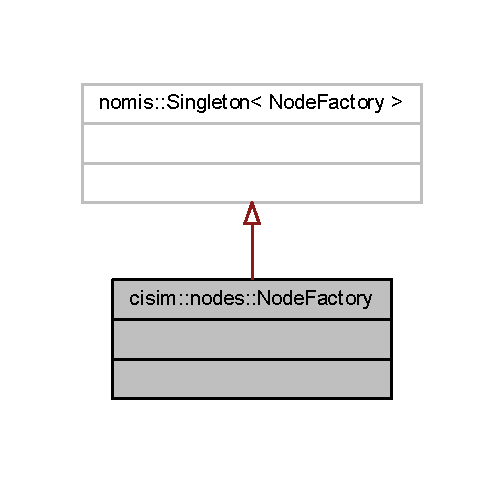
\includegraphics[width=242pt]{classcisim_1_1nodes_1_1_node_factory__inherit__graph}
\end{center}
\end{figure}


Collaboration diagram for cisim\+:\+:nodes\+:\+:Node\+Factory\+:\nopagebreak
\begin{figure}[H]
\begin{center}
\leavevmode
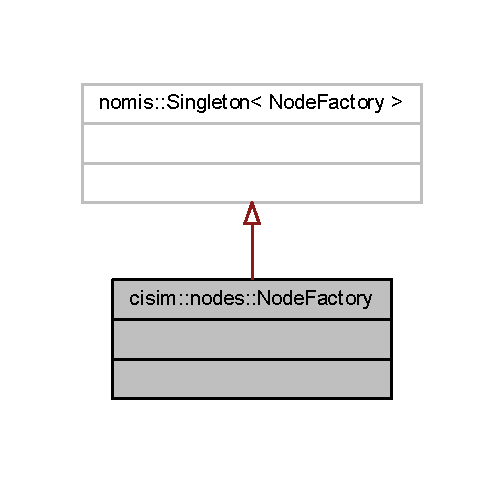
\includegraphics[width=242pt]{classcisim_1_1nodes_1_1_node_factory__coll__graph}
\end{center}
\end{figure}


The documentation for this class was generated from the following file\+:\begin{DoxyCompactItemize}
\item 
src/cisim/nodes/\hyperlink{nodefactory_8h}{nodefactory.\+h}\end{DoxyCompactItemize}

\hypertarget{classcisim_1_1nodes_1_1_node_registrar}{}\section{cisim\+:\+:nodes\+:\+:Node\+Registrar Class Reference}
\label{classcisim_1_1nodes_1_1_node_registrar}\index{cisim\+::nodes\+::\+Node\+Registrar@{cisim\+::nodes\+::\+Node\+Registrar}}


{\ttfamily \#include $<$noderegistrar.\+h$>$}



Collaboration diagram for cisim\+:\+:nodes\+:\+:Node\+Registrar\+:
\nopagebreak
\begin{figure}[H]
\begin{center}
\leavevmode
\includegraphics[width=220pt]{classcisim_1_1nodes_1_1_node_registrar__coll__graph}
\end{center}
\end{figure}


The documentation for this class was generated from the following file\+:\begin{DoxyCompactItemize}
\item 
src/cisim/nodes/\hyperlink{noderegistrar_8h}{noderegistrar.\+h}\end{DoxyCompactItemize}

\input{classcisim_1_1nodes_1_1_nor_node}
\input{classcisim_1_1nodes_1_1_not_node}
\input{classcisim_1_1nodes_1_1_or_node}
\input{classcisim_1_1nodes_1_1_xor_node}
\chapter{File Documentation}
\hypertarget{circuitsimulator_8cpp}{}\section{src/cisim/circuitsimulator.cpp File Reference}
\label{circuitsimulator_8cpp}\index{src/cisim/circuitsimulator.\+cpp@{src/cisim/circuitsimulator.\+cpp}}
{\ttfamily \#include \char`\"{}circuitsimulator.\+h\char`\"{}}\\*
Include dependency graph for circuitsimulator.\+cpp\+:\nopagebreak
\begin{figure}[H]
\begin{center}
\leavevmode
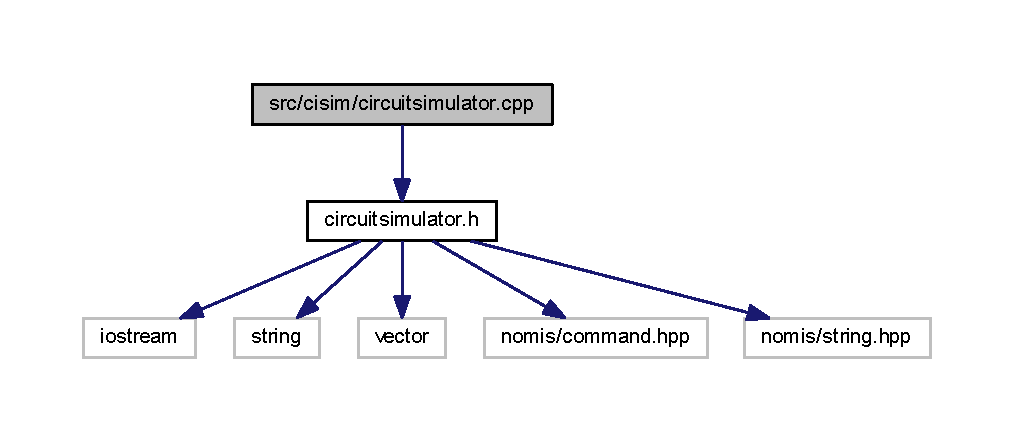
\includegraphics[width=350pt]{circuitsimulator_8cpp__incl}
\end{center}
\end{figure}

\hypertarget{circuitsimulator_8h}{}\section{src/cisim/circuitsimulator.h File Reference}
\label{circuitsimulator_8h}\index{src/cisim/circuitsimulator.\+h@{src/cisim/circuitsimulator.\+h}}
{\ttfamily \#include $<$iostream$>$}\\*
{\ttfamily \#include $<$string$>$}\\*
{\ttfamily \#include $<$vector$>$}\\*
{\ttfamily \#include \char`\"{}nomis/command.\+hpp\char`\"{}}\\*
{\ttfamily \#include \char`\"{}nomis/string.\+hpp\char`\"{}}\\*
Include dependency graph for circuitsimulator.\+h\+:\nopagebreak
\begin{figure}[H]
\begin{center}
\leavevmode
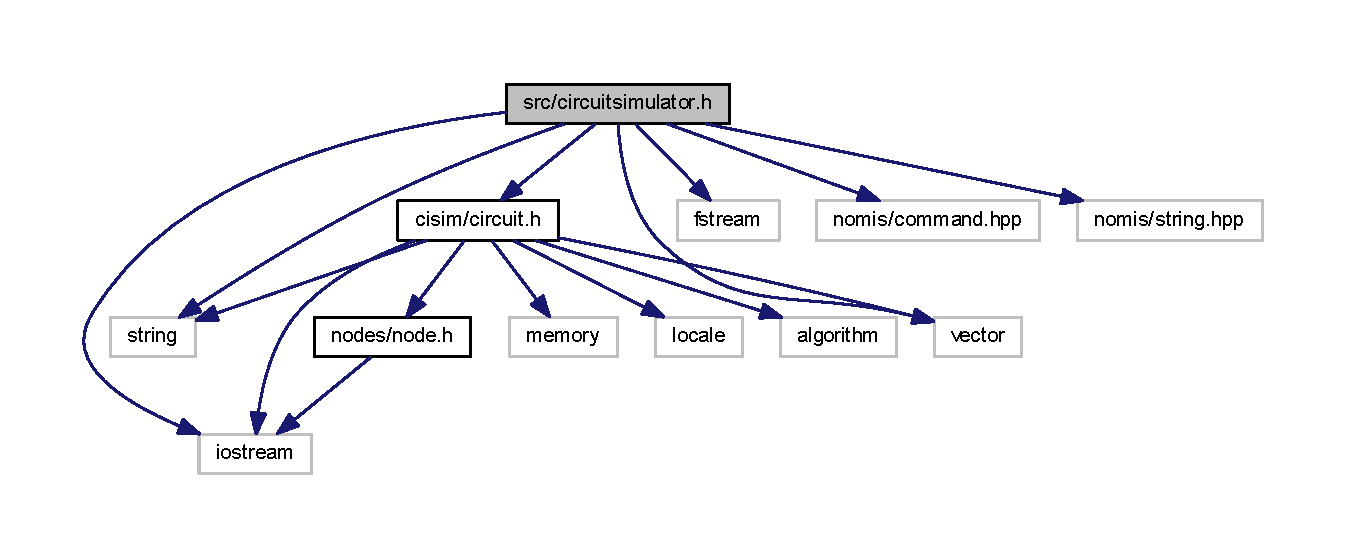
\includegraphics[width=350pt]{circuitsimulator_8h__incl}
\end{center}
\end{figure}
This graph shows which files directly or indirectly include this file\+:\nopagebreak
\begin{figure}[H]
\begin{center}
\leavevmode
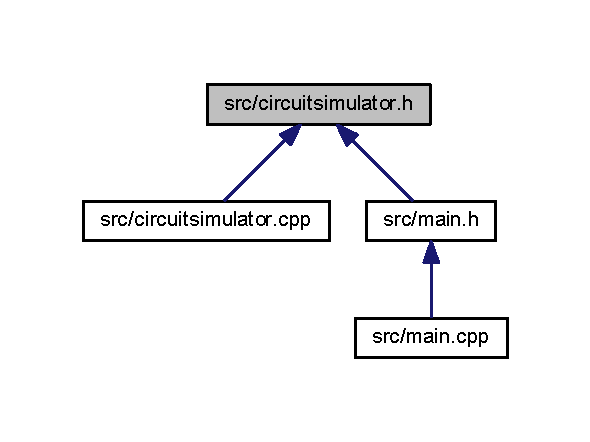
\includegraphics[width=336pt]{circuitsimulator_8h__dep__incl}
\end{center}
\end{figure}
\subsection*{Classes}
\begin{DoxyCompactItemize}
\item 
class \hyperlink{classcisim_1_1_circuit_simulator}{cisim\+::\+Circuit\+Simulator}
\begin{DoxyCompactList}\small\item\em Application class. \end{DoxyCompactList}\end{DoxyCompactItemize}
\subsection*{Namespaces}
\begin{DoxyCompactItemize}
\item 
 \hyperlink{namespacecisim}{cisim}
\end{DoxyCompactItemize}

\hypertarget{circuit_8cpp}{}\section{src/cisim/circuit.cpp File Reference}
\label{circuit_8cpp}\index{src/cisim/circuit.\+cpp@{src/cisim/circuit.\+cpp}}
{\ttfamily \#include \char`\"{}circuit.\+h\char`\"{}}\\*
Include dependency graph for circuit.\+cpp\+:
\nopagebreak
\begin{figure}[H]
\begin{center}
\leavevmode
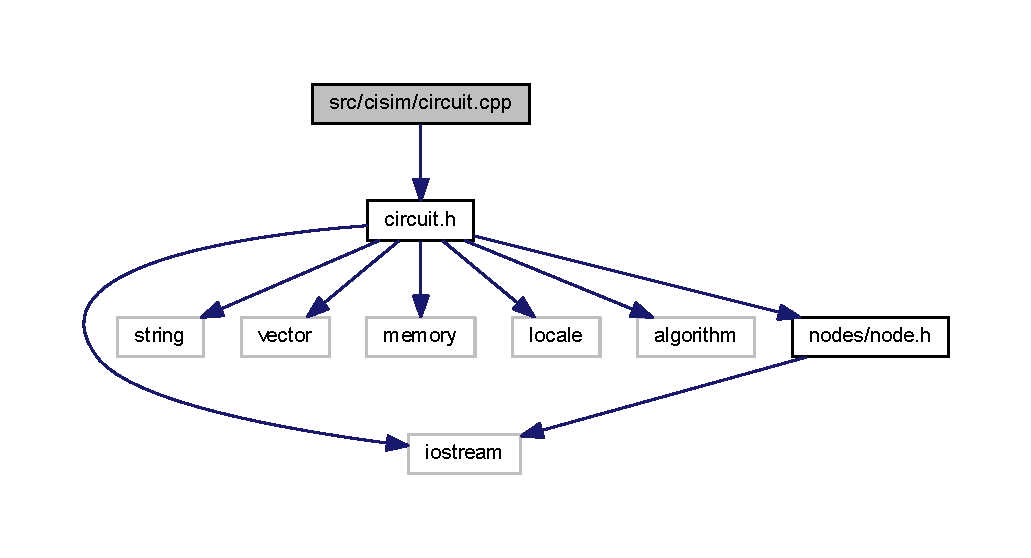
\includegraphics[width=350pt]{circuit_8cpp__incl}
\end{center}
\end{figure}

\hypertarget{circuit_8h}{}\section{src/cisim/circuit.h File Reference}
\label{circuit_8h}\index{src/cisim/circuit.\+h@{src/cisim/circuit.\+h}}
{\ttfamily \#include $<$iostream$>$}\\*
{\ttfamily \#include $<$string$>$}\\*
{\ttfamily \#include $<$vector$>$}\\*
{\ttfamily \#include $<$memory$>$}\\*
{\ttfamily \#include $<$locale$>$}\\*
{\ttfamily \#include $<$algorithm$>$}\\*
{\ttfamily \#include \char`\"{}nodes/node.\+h\char`\"{}}\\*
Include dependency graph for circuit.\+h\+:
\nopagebreak
\begin{figure}[H]
\begin{center}
\leavevmode
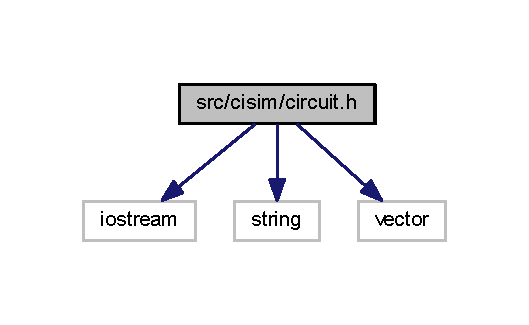
\includegraphics[width=350pt]{circuit_8h__incl}
\end{center}
\end{figure}
This graph shows which files directly or indirectly include this file\+:
\nopagebreak
\begin{figure}[H]
\begin{center}
\leavevmode
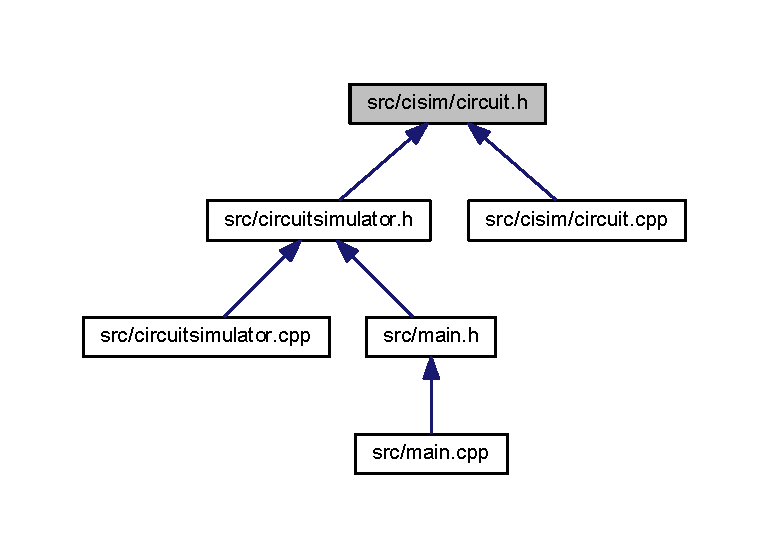
\includegraphics[width=350pt]{circuit_8h__dep__incl}
\end{center}
\end{figure}
\subsection*{Classes}
\begin{DoxyCompactItemize}
\item 
class \hyperlink{classcisim_1_1_circuit}{cisim\+::\+Circuit}
\begin{DoxyCompactList}\small\item\em \hyperlink{classcisim_1_1_circuit}{Circuit} class. \end{DoxyCompactList}\end{DoxyCompactItemize}
\subsection*{Namespaces}
\begin{DoxyCompactItemize}
\item 
 \hyperlink{namespacecisim}{cisim}
\end{DoxyCompactItemize}
\subsection*{Functions}
\begin{DoxyCompactItemize}
\item 
std\+::istream \& \hyperlink{namespacecisim_a9489303a86fdb03e3f7e13762bd748bd}{cisim\+::operator$>$$>$} (std\+::istream \&istream, Circuit \&circuit)
\end{DoxyCompactItemize}

\input{andnode_8h}
\input{inputnode_8h}
\input{nandnode_8h}
\hypertarget{node_8cpp}{}\section{src/cisim/nodes/node.cpp File Reference}
\label{node_8cpp}\index{src/cisim/nodes/node.\+cpp@{src/cisim/nodes/node.\+cpp}}
{\ttfamily \#include \char`\"{}node.\+h\char`\"{}}\\*
Include dependency graph for node.\+cpp\+:
\nopagebreak
\begin{figure}[H]
\begin{center}
\leavevmode
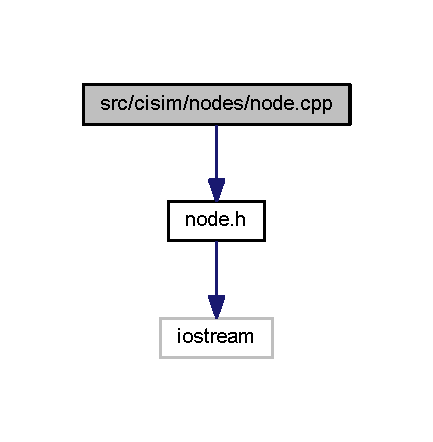
\includegraphics[width=208pt]{node_8cpp__incl}
\end{center}
\end{figure}

\hypertarget{node_8h}{}\section{src/cisim/nodes/node.h File Reference}
\label{node_8h}\index{src/cisim/nodes/node.\+h@{src/cisim/nodes/node.\+h}}
{\ttfamily \#include $<$iostream$>$}\\*
Include dependency graph for node.\+h\+:\nopagebreak
\begin{figure}[H]
\begin{center}
\leavevmode
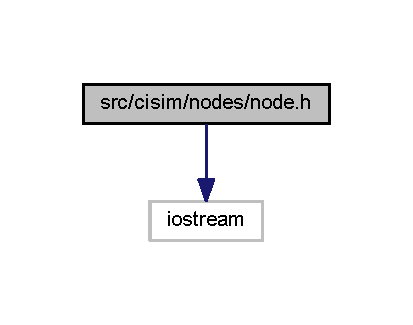
\includegraphics[width=198pt]{node_8h__incl}
\end{center}
\end{figure}
This graph shows which files directly or indirectly include this file\+:\nopagebreak
\begin{figure}[H]
\begin{center}
\leavevmode
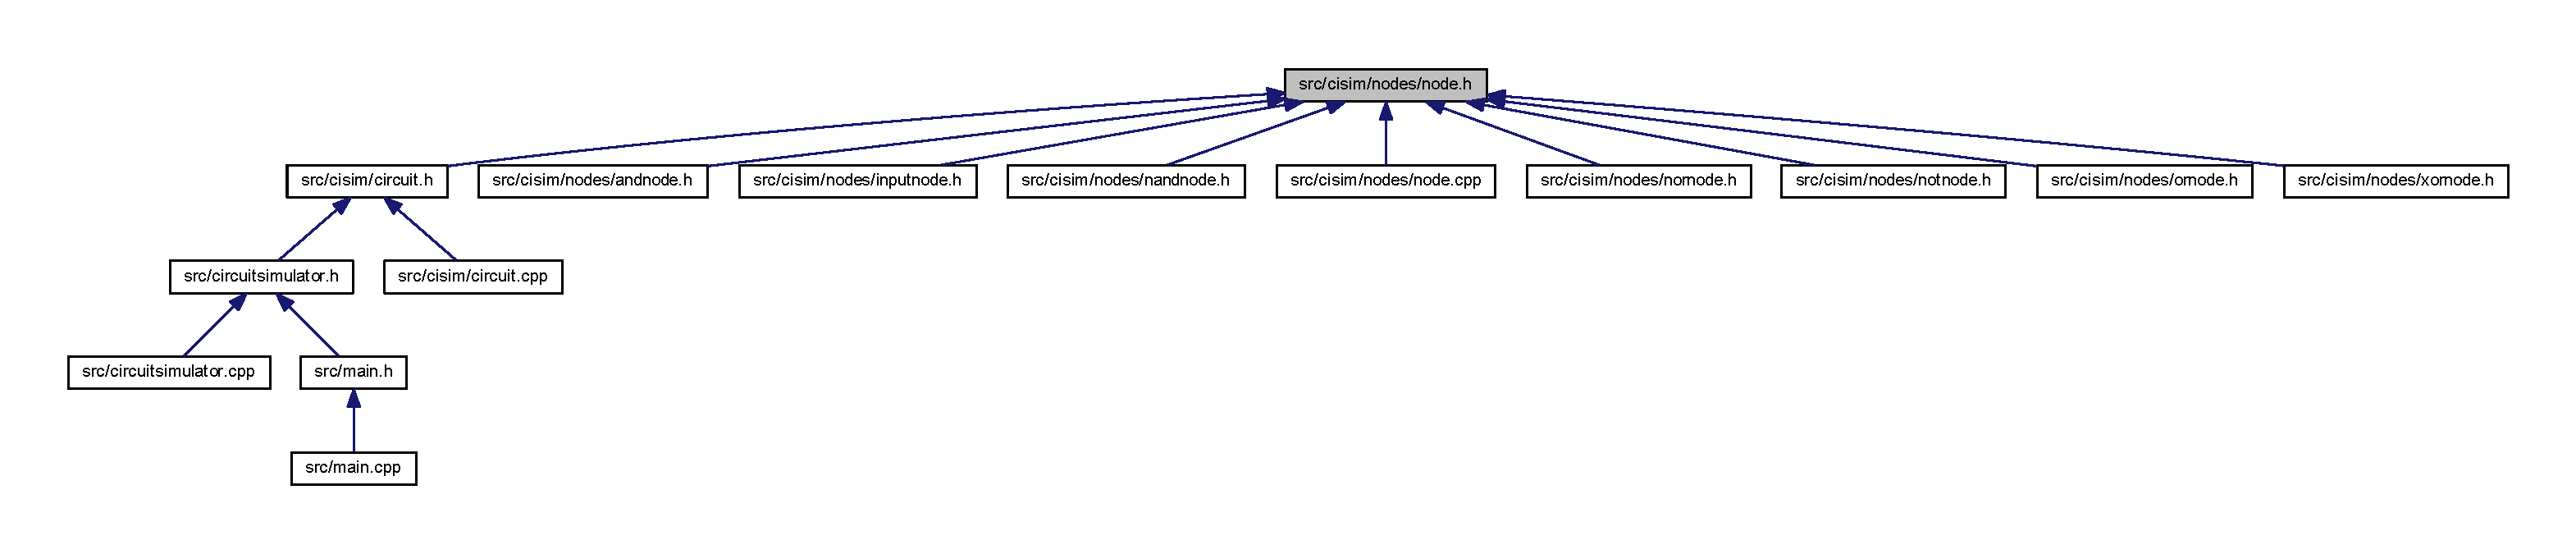
\includegraphics[width=208pt]{node_8h__dep__incl}
\end{center}
\end{figure}
\subsection*{Classes}
\begin{DoxyCompactItemize}
\item 
class \hyperlink{classcisim_1_1nodes_1_1_node}{cisim\+::nodes\+::\+Node}
\end{DoxyCompactItemize}
\subsection*{Namespaces}
\begin{DoxyCompactItemize}
\item 
 \hyperlink{namespacecisim}{cisim}
\item 
 \hyperlink{namespacecisim_1_1nodes}{cisim\+::nodes}
\end{DoxyCompactItemize}
\subsection*{Functions}
\begin{DoxyCompactItemize}
\item 
std\+::istream \& \hyperlink{namespacecisim_1_1nodes_a80da9ab6657bee6f2f7baa7e7cbc09ba}{cisim\+::nodes\+::operator$>$$>$} (std\+::istream \&istream, Node \&node)
\end{DoxyCompactItemize}

\hypertarget{nodefactory_8cpp}{}\section{src/cisim/nodes/nodefactory.cpp File Reference}
\label{nodefactory_8cpp}\index{src/cisim/nodes/nodefactory.\+cpp@{src/cisim/nodes/nodefactory.\+cpp}}
{\ttfamily \#include \char`\"{}nodefactory.\+h\char`\"{}}\\*
Include dependency graph for nodefactory.\+cpp\+:
\nopagebreak
\begin{figure}[H]
\begin{center}
\leavevmode
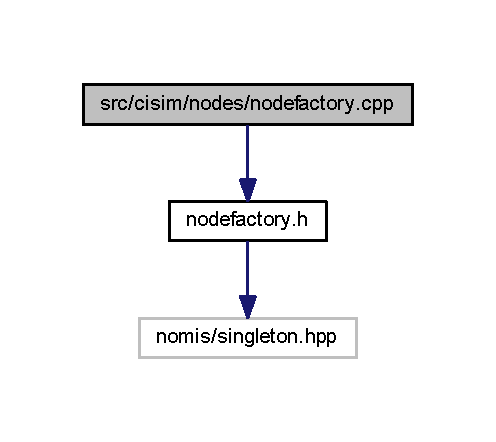
\includegraphics[width=238pt]{nodefactory_8cpp__incl}
\end{center}
\end{figure}

\hypertarget{nodefactory_8h}{}\section{src/cisim/nodes/nodefactory.h File Reference}
\label{nodefactory_8h}\index{src/cisim/nodes/nodefactory.\+h@{src/cisim/nodes/nodefactory.\+h}}
{\ttfamily \#include \char`\"{}nomis/singleton.\+hpp\char`\"{}}\\*
Include dependency graph for nodefactory.\+h\+:
\nopagebreak
\begin{figure}[H]
\begin{center}
\leavevmode
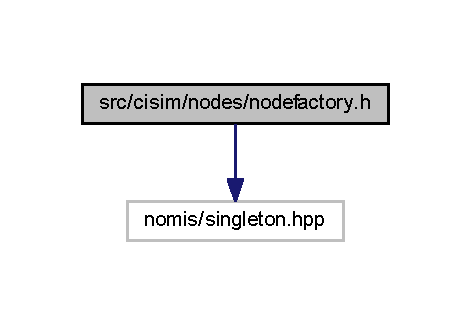
\includegraphics[width=226pt]{nodefactory_8h__incl}
\end{center}
\end{figure}
This graph shows which files directly or indirectly include this file\+:
\nopagebreak
\begin{figure}[H]
\begin{center}
\leavevmode
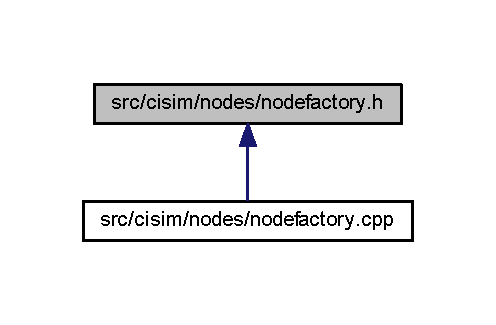
\includegraphics[width=238pt]{nodefactory_8h__dep__incl}
\end{center}
\end{figure}
\subsection*{Classes}
\begin{DoxyCompactItemize}
\item 
class \hyperlink{classcisim_1_1nodes_1_1_node_factory}{cisim\+::nodes\+::\+Node\+Factory}
\end{DoxyCompactItemize}
\subsection*{Namespaces}
\begin{DoxyCompactItemize}
\item 
 \hyperlink{namespacecisim}{cisim}
\item 
 \hyperlink{namespacecisim_1_1nodes}{cisim\+::nodes}
\end{DoxyCompactItemize}

\hypertarget{noderegistrar_8cpp}{}\section{src/cisim/nodes/noderegistrar.cpp File Reference}
\label{noderegistrar_8cpp}\index{src/cisim/nodes/noderegistrar.\+cpp@{src/cisim/nodes/noderegistrar.\+cpp}}
{\ttfamily \#include \char`\"{}noderegistrar.\+h\char`\"{}}\\*
Include dependency graph for noderegistrar.\+cpp\+:\nopagebreak
\begin{figure}[H]
\begin{center}
\leavevmode
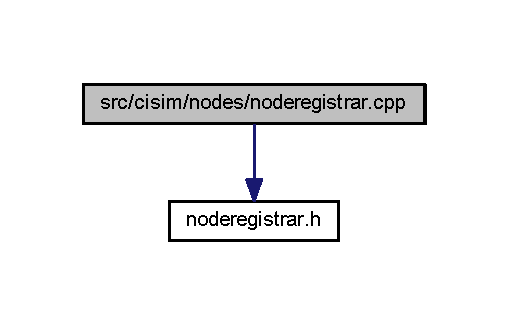
\includegraphics[width=244pt]{noderegistrar_8cpp__incl}
\end{center}
\end{figure}

\hypertarget{noderegistrar_8h}{}\section{src/cisim/nodes/noderegistrar.h File Reference}
\label{noderegistrar_8h}\index{src/cisim/nodes/noderegistrar.\+h@{src/cisim/nodes/noderegistrar.\+h}}
This graph shows which files directly or indirectly include this file\+:\nopagebreak
\begin{figure}[H]
\begin{center}
\leavevmode
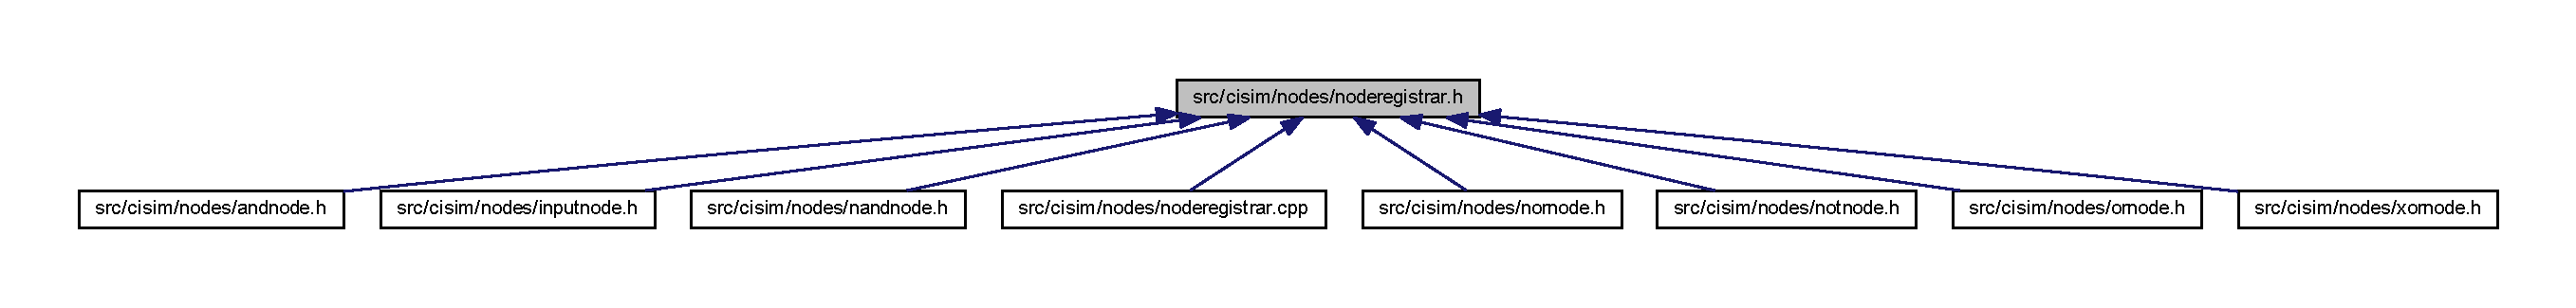
\includegraphics[width=244pt]{noderegistrar_8h__dep__incl}
\end{center}
\end{figure}
\subsection*{Classes}
\begin{DoxyCompactItemize}
\item 
class \hyperlink{classcisim_1_1nodes_1_1_node_registrar}{cisim\+::nodes\+::\+Node\+Registrar}
\end{DoxyCompactItemize}
\subsection*{Namespaces}
\begin{DoxyCompactItemize}
\item 
 \hyperlink{namespacecisim}{cisim}
\item 
 \hyperlink{namespacecisim_1_1nodes}{cisim\+::nodes}
\end{DoxyCompactItemize}

\input{nornode_8h}
\input{notnode_8h}
\input{ornode_8h}
\input{xornode_8h}
\hypertarget{main_8cpp}{}\section{src/main.cpp File Reference}
\label{main_8cpp}\index{src/main.\+cpp@{src/main.\+cpp}}
{\ttfamily \#include \char`\"{}main.\+h\char`\"{}}\\*
Include dependency graph for main.\+cpp\+:
\nopagebreak
\begin{figure}[H]
\begin{center}
\leavevmode
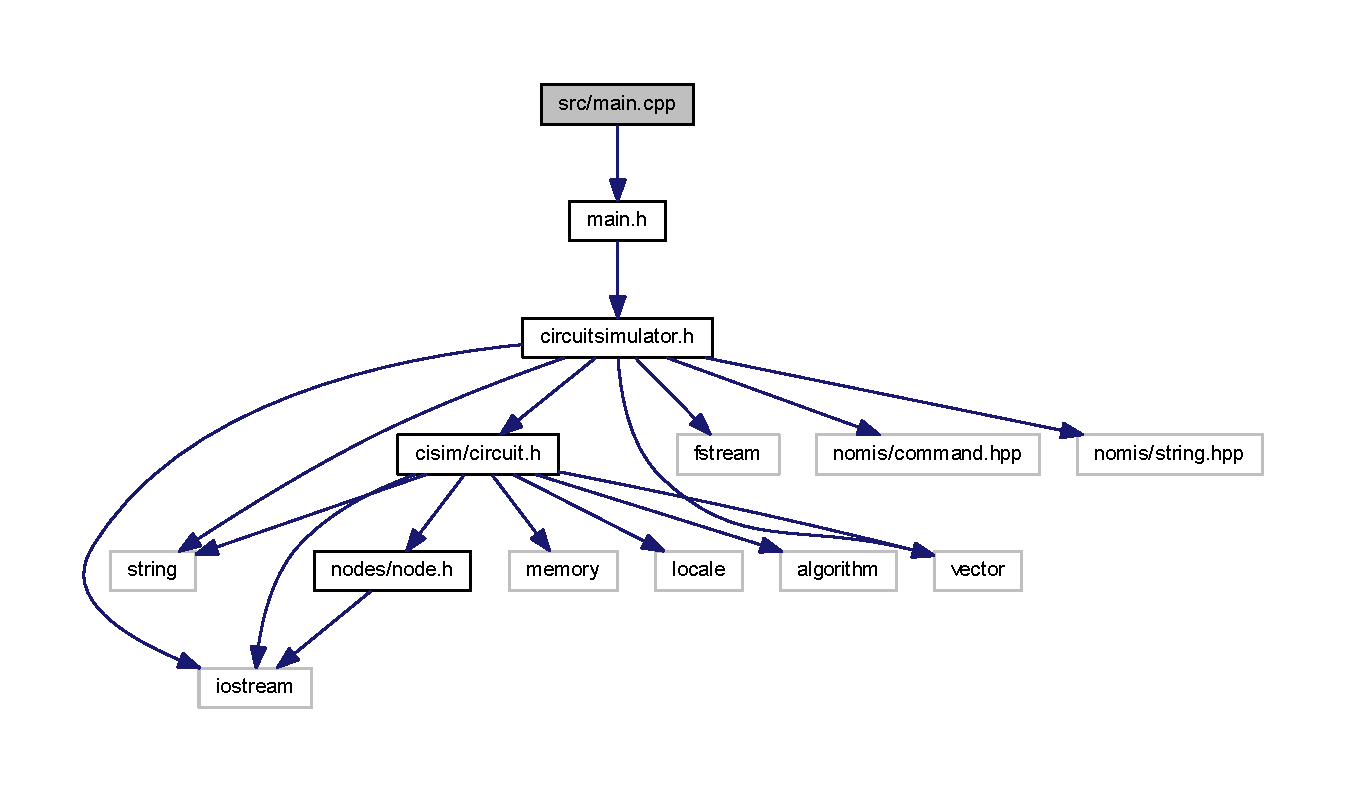
\includegraphics[width=350pt]{main_8cpp__incl}
\end{center}
\end{figure}
\subsection*{Functions}
\begin{DoxyCompactItemize}
\item 
int \hyperlink{main_8cpp_ae66f6b31b5ad750f1fe042a706a4e3d4}{main} ()
\end{DoxyCompactItemize}


\subsection{Function Documentation}
\index{main.\+cpp@{main.\+cpp}!main@{main}}
\index{main@{main}!main.\+cpp@{main.\+cpp}}
\subsubsection[{\texorpdfstring{main()}{main()}}]{\setlength{\rightskip}{0pt plus 5cm}int main (
\begin{DoxyParamCaption}
{}
\end{DoxyParamCaption}
)}\hypertarget{main_8cpp_ae66f6b31b5ad750f1fe042a706a4e3d4}{}\label{main_8cpp_ae66f6b31b5ad750f1fe042a706a4e3d4}

\hypertarget{main_8h}{}\section{src/main.h File Reference}
\label{main_8h}\index{src/main.\+h@{src/main.\+h}}
{\ttfamily \#include \char`\"{}circuitsimulator.\+h\char`\"{}}\\*
Include dependency graph for main.\+h\+:
\nopagebreak
\begin{figure}[H]
\begin{center}
\leavevmode
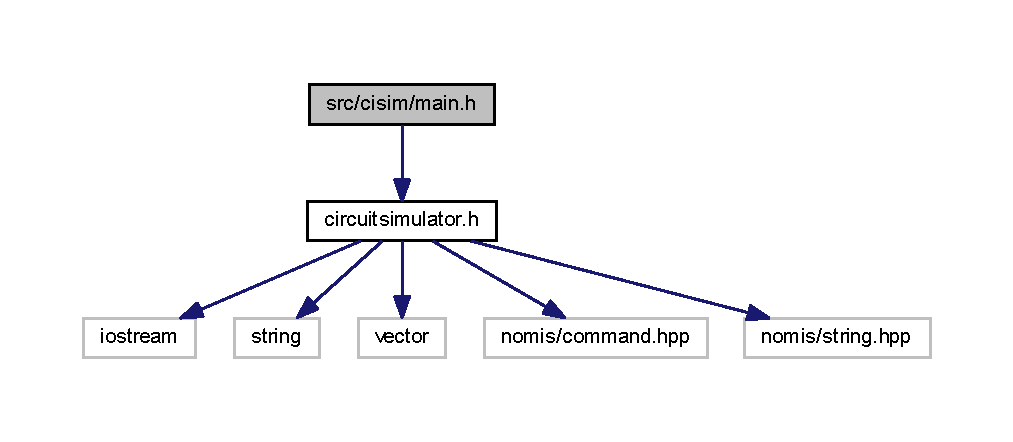
\includegraphics[width=350pt]{main_8h__incl}
\end{center}
\end{figure}
This graph shows which files directly or indirectly include this file\+:\nopagebreak
\begin{figure}[H]
\begin{center}
\leavevmode
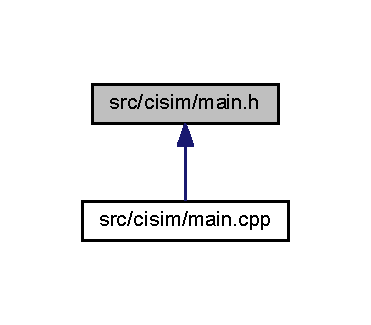
\includegraphics[width=152pt]{main_8h__dep__incl}
\end{center}
\end{figure}

%--- End generated contents ---

% Index
\backmatter
\newpage
\phantomsection
\clearemptydoublepage
\addcontentsline{toc}{chapter}{Index}
\printindex

\end{document}
